\section{New results: legal consumption without an outcome advantage}
\label{sec:abc-results}
\subsection{All three assigned arms reach the correct scientific decision}
Table~\ref{tab:abc-outcomes} uses all eighteen frozen attempts. Each arm
has six actual decision artifacts, six correct predictions, six correct
adopt/retain decisions and six independent selected-service passes. All
intervention predictions have coverage. There are no wrong adoptions or
rejections. Every context rejects the storage and reset interventions and
adopts the passing package intervention. The complete-information baseline
therefore leaves no observed scientific-accuracy deficit for refinement to
remove on this finite task list~\cite{abcb,abcreview}.

\begin{table}[tbp]
\centering\small
\setlength{\tabcolsep}{4.5pt}
\caption{New formal outcomes, each out of six assigned attempts (three tasks, two fresh contexts each). Actual submission is distinct from normal budget completion. Pred., Dec. and Svc. denote correct intervention prediction, correct adopt/retain decision and selected-service PASS. Typed is only a path statistic.}
\label{tab:abc-outcomes}
\begin{tabular}{lrrrrrr}
\toprule
Assigned arm & Actual sub. & Pred. & Dec. & Svc. & Budget & Typed \\
\midrule
Complete information & 6/6 & 6/6 & 6/6 & 6/6 & 6/6 & 1/6 \\
Fixed conservative rules & 6/6 & 6/6 & 6/6 & 6/6 & 4/6 & 4/6 \\
Observation refinement & 6/6 & 6/6 & 6/6 & 6/6 & 6/6 & 3/6 \\
\bottomrule
\end{tabular}
\end{table}


Normal budget completion is a separate outcome. Complete information and
refinement each finish normally in six attempts; fixed rules finish normally
in four. The first fixed-rule repeats on reset placement and package response
each reach twelve settled requests and retain
\path{INCOMPLETE_OR_STOPPED}. Before stopping, both have an actual direct
submission with a correct prediction and decision and selected-service PASS.
They are neither missing submissions nor normally completed episodes. Their
full costs and the original stop labels remain in the table denominator.

Actual typed consumption occurs in one complete-information attempt, four
fixed-rule attempts and three refinement attempts. The other decisions are
legal direct submissions. In particular, three refinement attempts do not
complete the proposed typed path but do reach the correct engineering
decision. They remain in the assigned refinement arm; no replacement episode
is run. The 1/4/3 counts describe use of an optional path, not relative
scientific success. Applying the path-specific conjunction to all arms would
incorrectly penalize a strong direct baseline.

\subsection{What a formal typed observation establishes}
The refinement reset example binds event/contact and transmission timing from
complete inputs to the shunt time in the excitation source. Its Boolean result
is false and is actually read by the retain branch. The stored edge identifies
both source hashes, the typed value and the executed current-input hash.
The independent saved trajectories then establish why retain passes and adopt
fails: the 12.1 ms intervention reset clears the volatile event after the
contact ends, whereas the current input sends before its late reset.

The passing package example also consumes a Boolean, now true, and selects
adopt. Its proposed relation combines pulse start, deadline, boot delay, TX
duration, power and efficiency with the energy needed to reach the ready
threshold. The independent executor supplies the actual 98.7 ms reception.
The source calculation is a qualified intermediate fact; the final service
check additionally covers event availability, loads and reception. Correct
service on this one input does not prove that the proxy is sufficient over
every numeric bound in its declared domain.

The storage example consumes false and retains parallel storage. Its
energy-window proxy correctly accompanies that decision on the frozen input,
but does not replace the full transient model. In particular, harvest during
TX, boot-step overshoot and the ESR guard must be considered before promoting
such a proxy to an exact criterion. The raw proposal and its explanatory
text are retained as participant outputs; interpreter agreement and a correct
selected outcome do not validate every explanatory statement. No formal
attempt supplies a new physical measurement or establishes universal
autonomous discovery~\cite{abcb,abcaudit}.

\subsection{More requests, equal acquisition and a mixed cost result}
Table~\ref{tab:abc-costs} shows 37, 59 and 50 requests for complete information,
fixed rules and refinement. Each acquires exactly 89,218 logical source bytes
over six attempts. Refinement therefore has no observed acquisition-volume
gain and uses thirteen more requests than complete information. Preflight
calls number 15/34/20 and rejected actions 9/27/14. Improving the admission
schema does not remove operational errors or make extra interaction free.

\begin{table}[tbp]
\centering\small
\setlength{\tabcolsep}{4.5pt}
\caption{New formal resource totals over six attempts per arm. Tokens are total input/output usage; reasoning tokens are not added a second time. USD is the conservative fixed-rate estimate, not an invoice. Acquired bytes are logical source-response bytes, not disk I/O or total context volume.}
\label{tab:abc-costs}
\begin{tabular}{lrrrrr}
\toprule
Assigned arm & Requests & Input tokens & Output tokens & Est. USD & Acquired B \\
\midrule
Complete information & 37 & 1,207,152 & 198,172 & 0.5999520 & 89,218 \\
Fixed conservative rules & 59 & 1,816,101 & 226,434 & 0.8165511 & 89,218 \\
Observation refinement & 50 & 1,157,649 & 176,741 & 0.5593839 & 89,218 \\
\bottomrule
\end{tabular}
\end{table}


The corresponding conservative fee estimates are USD~0.5999520, 0.8165511
and 0.5593839. The calculation uses input and output usage at fixed rates:
\begin{equation}
 \widehat C_{\rm USD}
 =0.30\frac{N_{\rm input}}{10^6}
  +1.20\frac{N_{\rm output}}{10^6}.
\end{equation}
Reasoning tokens are an output-accounting field, not an additional additive
budget. Refinement uses fewer total input and output tokens than complete
information in these receipts despite its larger request count. That yields
the slightly lower fee estimate; it does not make every cost dimension better.
Rates, response length and initial payload volume all enter this descriptive
comparison. The estimates are not invoices and exclude unmetered preparation.

\begin{figure}[tbp]
\centering
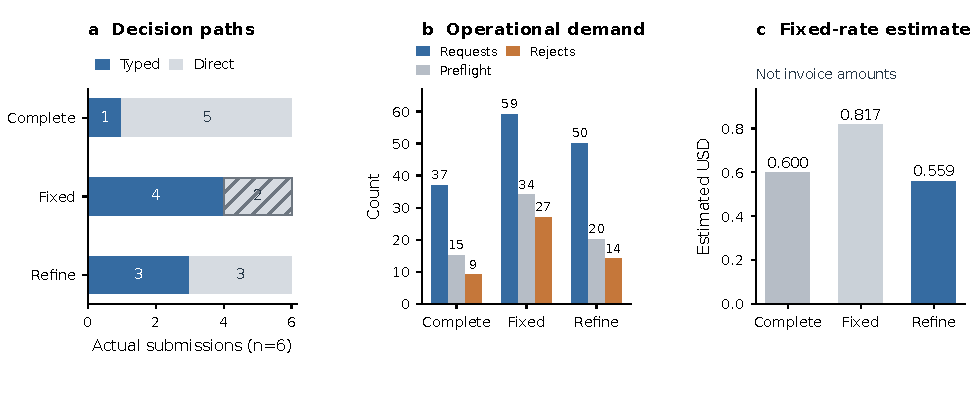
\includegraphics[width=\linewidth]{figures/cost-paths.pdf}
\caption{New formal path and cost comparison, all six assigned attempts per
arm. (a) Typed and direct submissions both count as actual artifacts; hatching
marks the two fixed-rule budget stops after direct submission. (b) Requests,
preflights and rejects are distinct operational counts. (c) Conservative
fixed-rate fees, rounded here to three decimals. All arms independently have
six correct predictions, six correct decisions and six selected-service passes.
Bars are finite totals across three fixed tasks and two fresh contexts per
task; no error bars, significance or population estimate is implied.}
\label{fig:abc-costs}
\end{figure}

\begin{table}[tbp]
\centering\small
\setlength{\tabcolsep}{4.5pt}
\caption{Operational and execution accounting. Initial B is summed initial payload bytes; PF/rej. count preflights/rejected actions. Wall includes host evaluation; no separate host-only duration was recorded. Eval/cache/new count evaluated-input references, cache hits and new scientific computations, respectively. Cache order prevents an algorithmic-savings interpretation.}
\label{tab:abc-accounting}
\begin{tabular}{lrrrrrrrr}
\toprule
Arm & Initial B & PF & Rej. & Tool s & Wall s & Eval & Cache & New \\
\midrule
Complete & 175,414 & 15 & 9 & 0.376 & 870.3 & 12 & 8 & 4 \\
Fixed & 62,054 & 34 & 27 & 0.162 & 926.7 & 12 & 12 & 0 \\
Refine & 61,850 & 20 & 14 & 0.176 & 755.7 & 12 & 12 & 0 \\
\bottomrule
\end{tabular}
\end{table}


All arms have twelve evaluated-input references. Complete information accounts
for four new scientific computations and eight cache reuses; fixed rules and
refinement each reuse twelve cached inputs and add zero computations. Five
distinct exact inputs underlie the three mechanisms because two tasks share
the same current design. The cache is warmer for later arms, so the zero is
not an algorithmic compute saving. Tool time is separately reported from
total wall time, and the unrecorded host-only duration remains unavailable.

The B formal batch totals 146 settled requests, USD~1.9758870 in these
estimates and 2552.7 summed episode seconds. The complete finite cycle has
48 model episodes and 307 settled requests with an estimate of
USD~5.5299957; this already includes B, A and C formation/validation/formal
work and must not be added to their subtotals. The developer rehearsal has
zero model requests and remains outside eighteen~\cite{abcb,abcaudit}.

\begin{table}[tbp]
\centering\small
\setlength{\tabcolsep}{4.5pt}
\caption{Every new formal attempt, with no deletion or replacement. C/F/R denote complete information, fixed rules and refinement. S is normal ACTUAL\_SUBMITTED completion; X is original INCOMPLETE\_OR\_STOPPED. Every row has an actual artifact, correct prediction/decision and selected-service PASS; T indicates actual typed use.}
\label{tab:abc-attempts}
\begin{tabular}{lrrrrrrr}
\toprule
Mechanism & Arm & Repeat & Status & T & Requests & PF & Rejects \\
\midrule
package response & C & 1 & S & 0 & 7 & 3 & 2 \\
package response & C & 2 & S & 0 & 7 & 4 & 3 \\
package response & F & 1 & X & 0 & 12 & 9 & 7 \\
package response & F & 2 & S & 1 & 11 & 6 & 5 \\
package response & R & 1 & S & 1 & 6 & 3 & 2 \\
package response & R & 2 & S & 0 & 10 & 5 & 4 \\
reset placement & C & 1 & S & 0 & 4 & 2 & 1 \\
reset placement & C & 2 & S & 0 & 6 & 2 & 1 \\
reset placement & F & 1 & X & 0 & 12 & 8 & 7 \\
reset placement & F & 2 & S & 1 & 6 & 2 & 1 \\
reset placement & R & 1 & S & 0 & 10 & 4 & 2 \\
reset placement & R & 2 & S & 1 & 8 & 2 & 1 \\
storage connection & C & 1 & S & 1 & 7 & 2 & 1 \\
storage connection & C & 2 & S & 0 & 6 & 2 & 1 \\
storage connection & F & 1 & S & 1 & 10 & 6 & 5 \\
storage connection & F & 2 & S & 1 & 8 & 3 & 2 \\
storage connection & R & 1 & S & 1 & 7 & 3 & 2 \\
storage connection & R & 2 & S & 0 & 9 & 3 & 3 \\
\bottomrule
\end{tabular}
\end{table}


\subsection{Relation to the earlier negative comparison}
The new protocol establishes actual legal consumption under frozen new
mechanisms and preserves all original source/type failures. It does not
retroactively change the earlier seven-pass/five-incomplete E5 result, and
the new six-per-arm scientific outcome cannot be read as a controlled
before/after effect of preflight: task list, resource limits and protocol
version differ. Both studies support the same bounded comparison. Complete
static information is a successful control, and the live refinement route
has not demonstrated additional scientific success. The new study further
shows equal source acquisition, more requests than the strongest control,
and a mixed rather than comprehensive cost advantage.
\FloatBarrier
